\subsection{Chapter Overview}

\subsection{CLEMAP Client Dataset}

The client of CLEMAP operates within the Swiss printing and media industry where the equipment has been fitted with state of the art CLEMAP sensors on a range of their production equipment. The machines, location, and purpose are described in Table 1:

\begin{table}[htbp]
    \renewcommand{\arraystretch}{1.2}
    \centering
    \begin{tabular}{lcccccc}
    \hline
         Machine/Component & System & Amperes & Location & Floor & Purpose  \\
    \hline
    Gesamtmessung & & 1600 & Bau II & 0 & Main terminal \\
    Hauptluftung & HVAC & 250 & Bau II & -1 & Main ventilation \\
    Kältemaschiene & & 200 & Bau II & 1 & Refrigeration \\
    Drückmaschine & XL106 & 315 & Bau II & 2 & Printer \\
    UV Scan & XL106 & 160 & Bau II & 1 & undefined \\
    UV Sigmaline EG & & 315 & Bau II & 0 & undefined \\
    Stahl Folder & & 63 & Bau II & 0 & Steel folding \\
    Puderabsauger & R707LV & 25 & Bau II & 2 & Powder extraction \\
    Vari Air & R707LV & 100 & Bau II & 2 & undefined \\
    Trockner & R707LV & 160 & Bau II & 2 & Dryer \\
    UV Feinabgäng & & 125 & Bau II & 0 & UV fine particle extractor \\
    Papier Entsorgung & & 125 & Bau II & -1 & Paper disposal \\
    UV 1.0G & & 125 & Bau II & 1 & UV server room \\
    UV 2.0G & & 125 & Bau II & 2 & $2^{nd}$ floor \\
    UV 3.0G & & 125 & Bau II & 3 & $3^{rd}$ floor \\
    UV 4.0G & & 160 & Bau II & 4 & $4^{th}$ floor \\
    UV EG & & 125 & Bau II & 0 & UV ground floor \\
    \hline
    \end{tabular}
    \caption{List of items being metered by CLEMAP. A system may be composed of several machines, all of which are being metered.}
    \label{tab:my_label}
\end{table}

All machines and the main terminals are connected to an alternating current (AC) grid with three phases. Subsequently, the data collected is the phase, voltage (V), current (I), \textbf{s}, power (Watts), \textbf{q}, power factor (PF), \textbf{phi}. The measurements were originally collected at a frequency of $12$ hertz (Hz) from October $7^{th}$ until October $18^{th}$ for a total length of $10$ days. A three phase current at $12$Hz indicates that every second, there should be $12$ cycles being measured for each phase $1, 2$ and $3$. 

As outlined in \hyperlink{subsection.3.3}{section 3.3}, and due to the GPyTorch Gaussian Process time complexity of $\mathcal{O}(n^2)$, the time series is discretized by aggregating the data into $10$ and $30$ minute intervals and taking the average value. This aggregation significantly reduces the length of the time series while still allowing for a more granular level of analysis compared to the current literature in \hyperlink{subsection.2}{section 2}.

\subsubsection{CLEMAP Exploratory Data Analysis}

Here, an introductory exploratory data analysis (EDA) is performed on some of the machines and components that will be modeled in \hyperlink{subsection.5}{section 5}. First, a bar plot broken down by machine energy consumption and hour of the day for the $10$ days is visualized for a general overview of the measurement setup.

\begin{figure}[htp]
\centering
\graphicspath{ {./images/} }
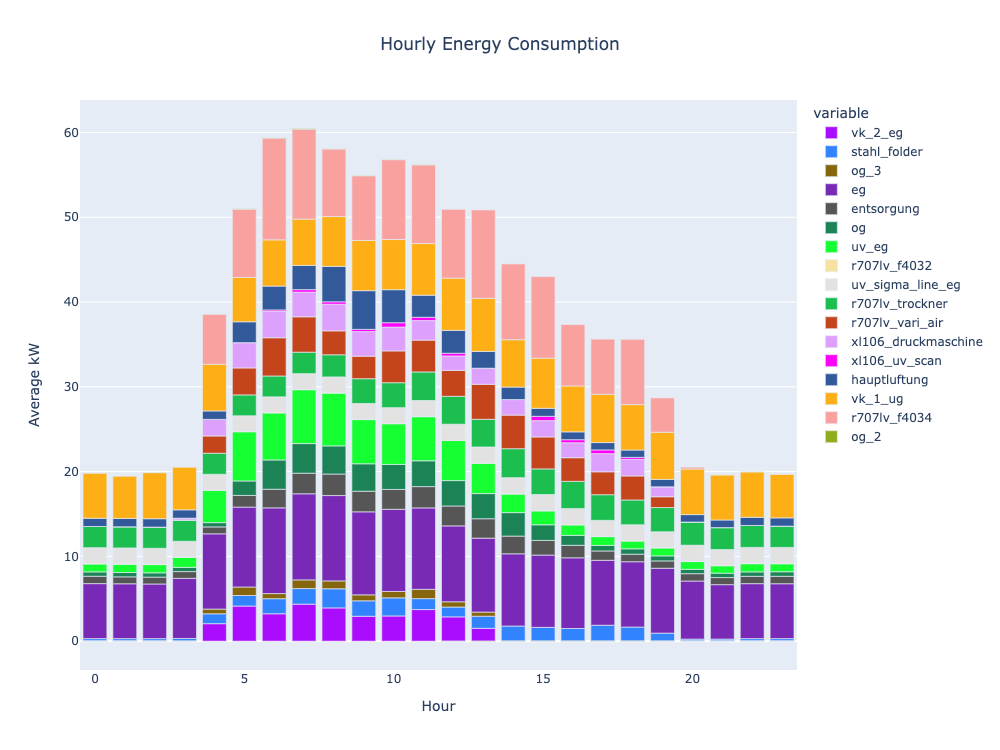
\includegraphics[scale=0.41]{images/hourly_load_barplot.png}
\caption{CLEMAP sensor measurement setup. Hourly load energy consumption (kWh) for each machine over the course of $10$ days.}
\end{figure}

Using the meta data from \hyperlink{table.1}{Table 1} and the bar chart above, it is evident that machines on the ground, first, and second floor effect the energy being metered on their respective floors (UV 1.0G, etc.). Likewise, the meter on the main terminal is measuring all of the energy. 

Consist energy use / always on = UV Sigma line, trockner, HVAC,  VK 1.UG, entsorgung


More variable / effected by hour of day = vk 2.eg, stahl folder, og 3,  og, uv eg, r707lv f4032, vari air, druckmaschine, xl106 uv scan, r707lv f4032, og 2


The three main systems; (1) HVAC, (2) XL106, and (3) R707LV 

For the sake of brevity, only the EDA for the paper disposal machine (\hyperlink{figure.6}{Figure 7}) will be shown below. For a full machine analysis, please refer to the \textit{eda} directory of the GitHub repository \cite{GitHub}. 

\begin{figure}[h]
  \centering
  \graphicspath{ {./images/} }
  \subfloat[Outside of machine.]{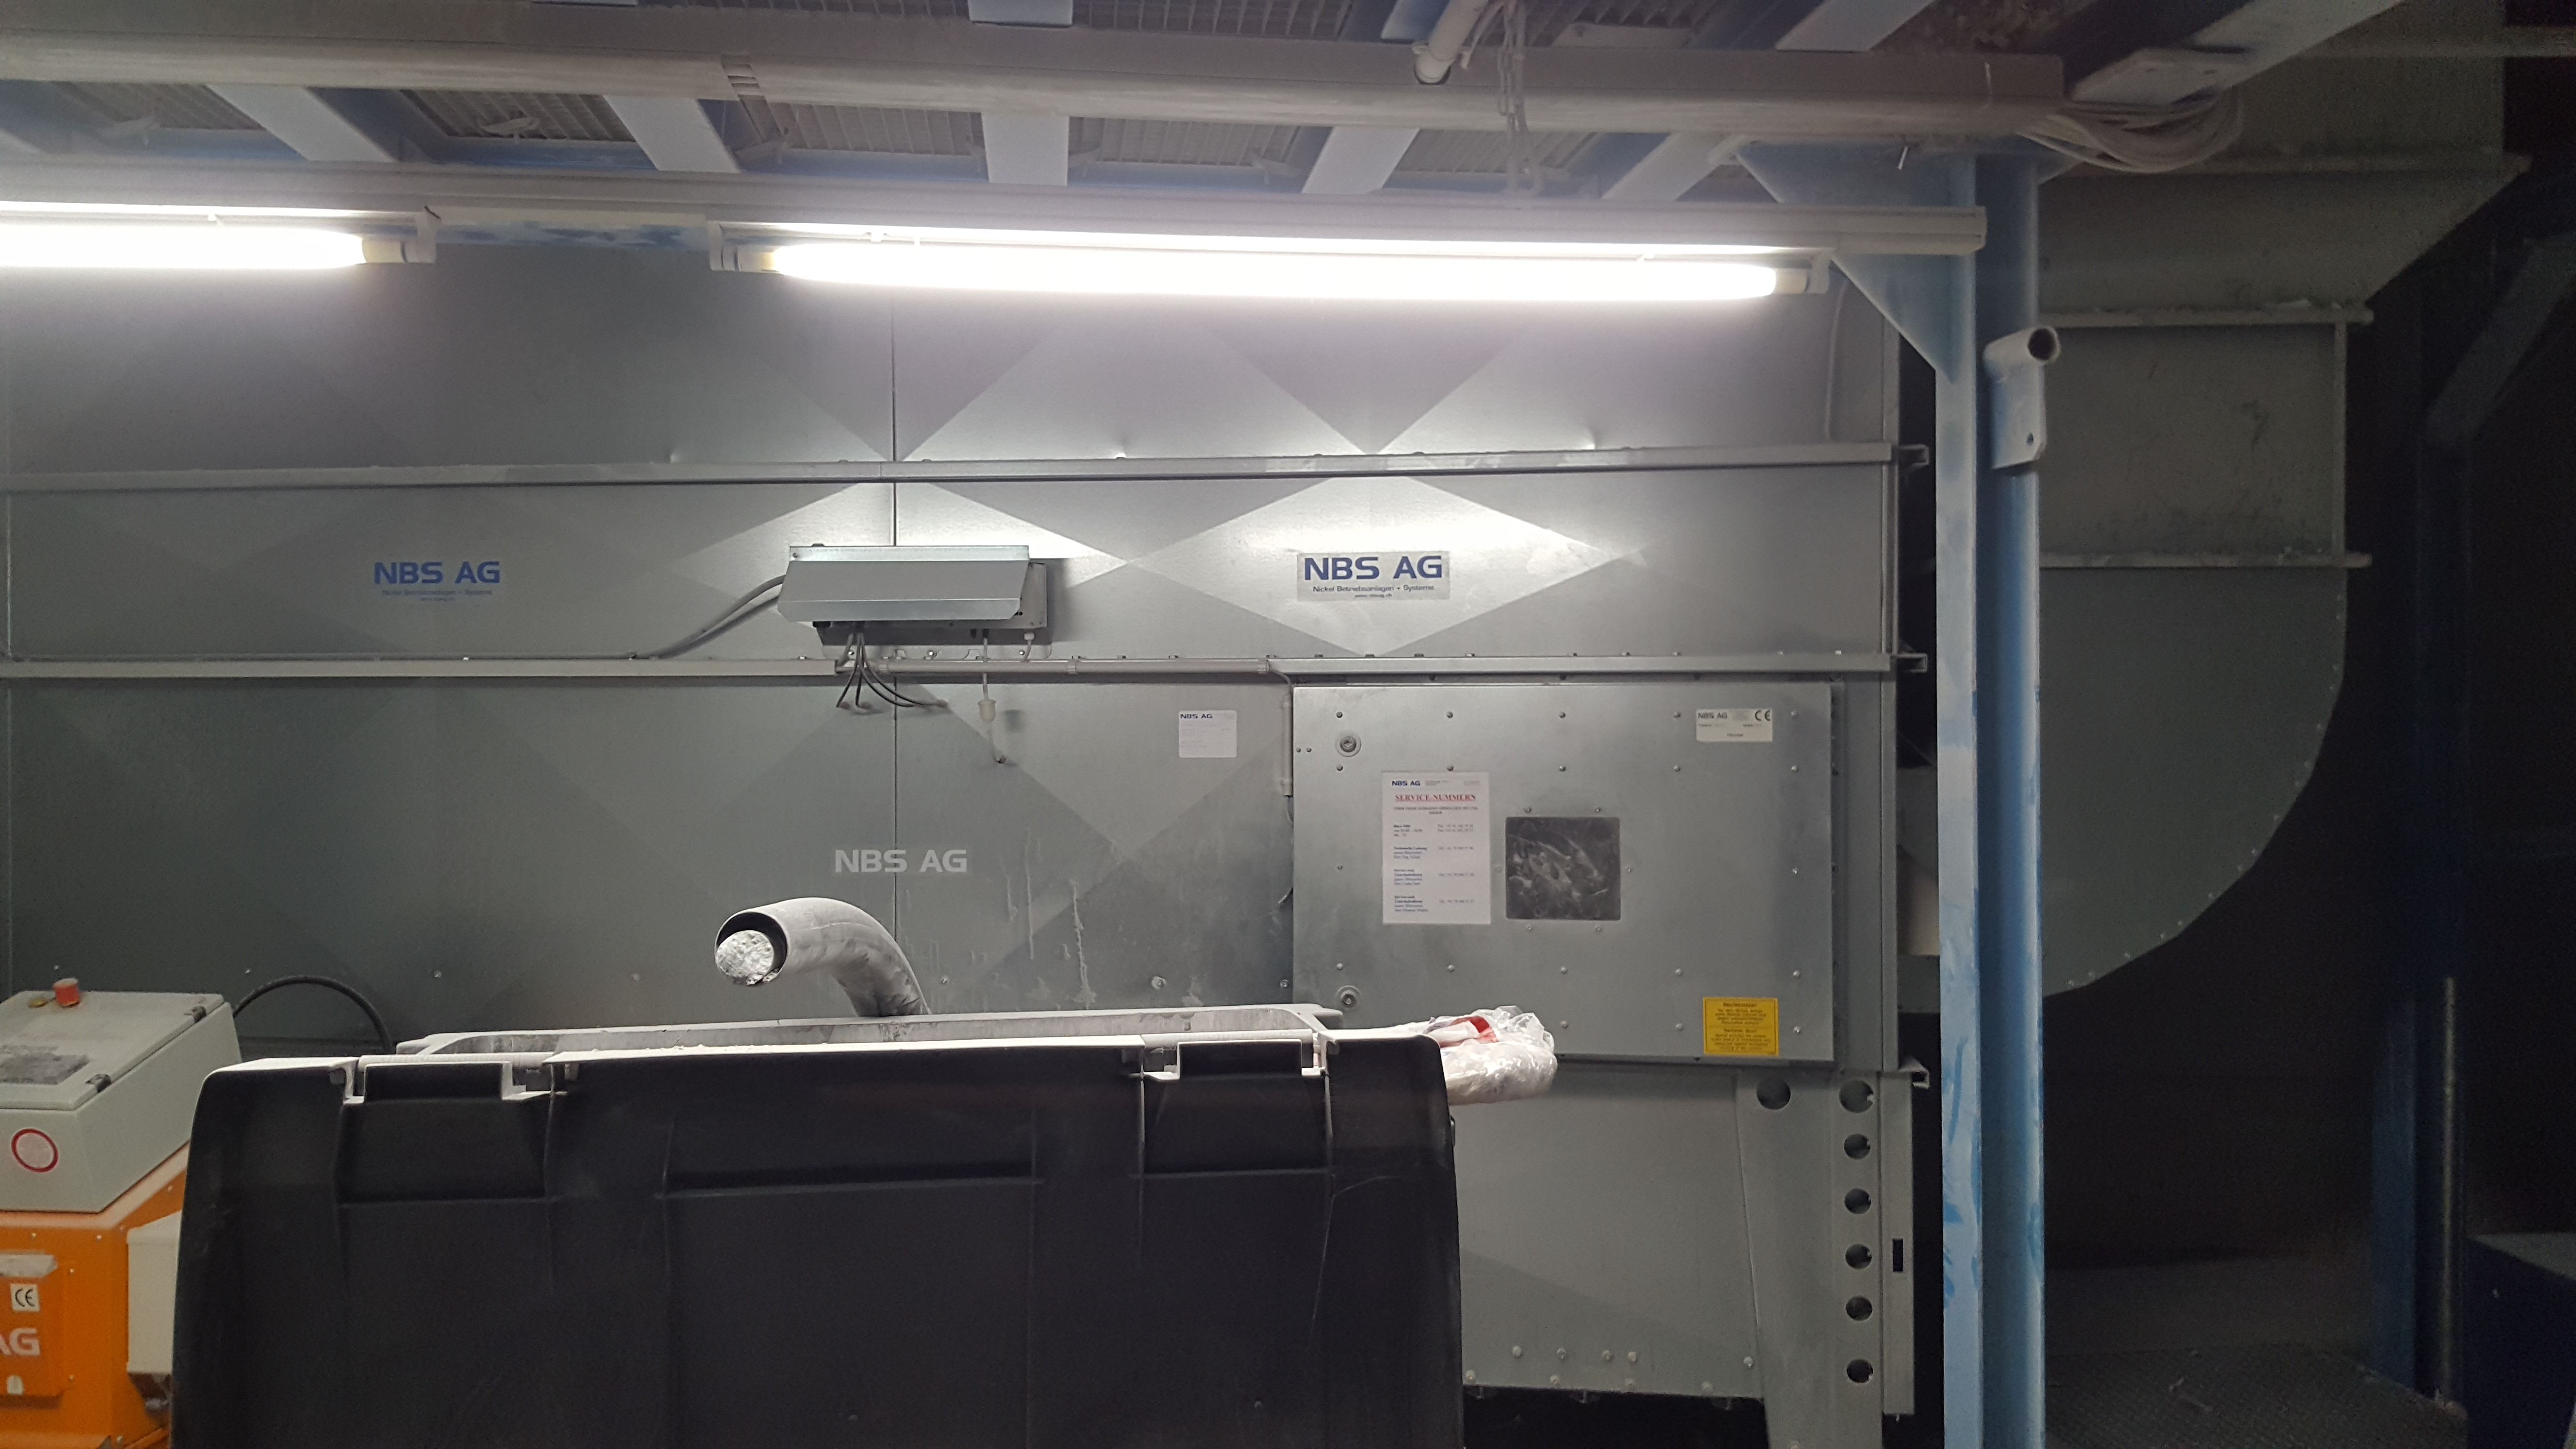
\includegraphics[width=0.4\textwidth]{images/papier_entsorgung_1.jpg}\label{fig:f1}}
  \hfill
  \subfloat[Output of machine.]{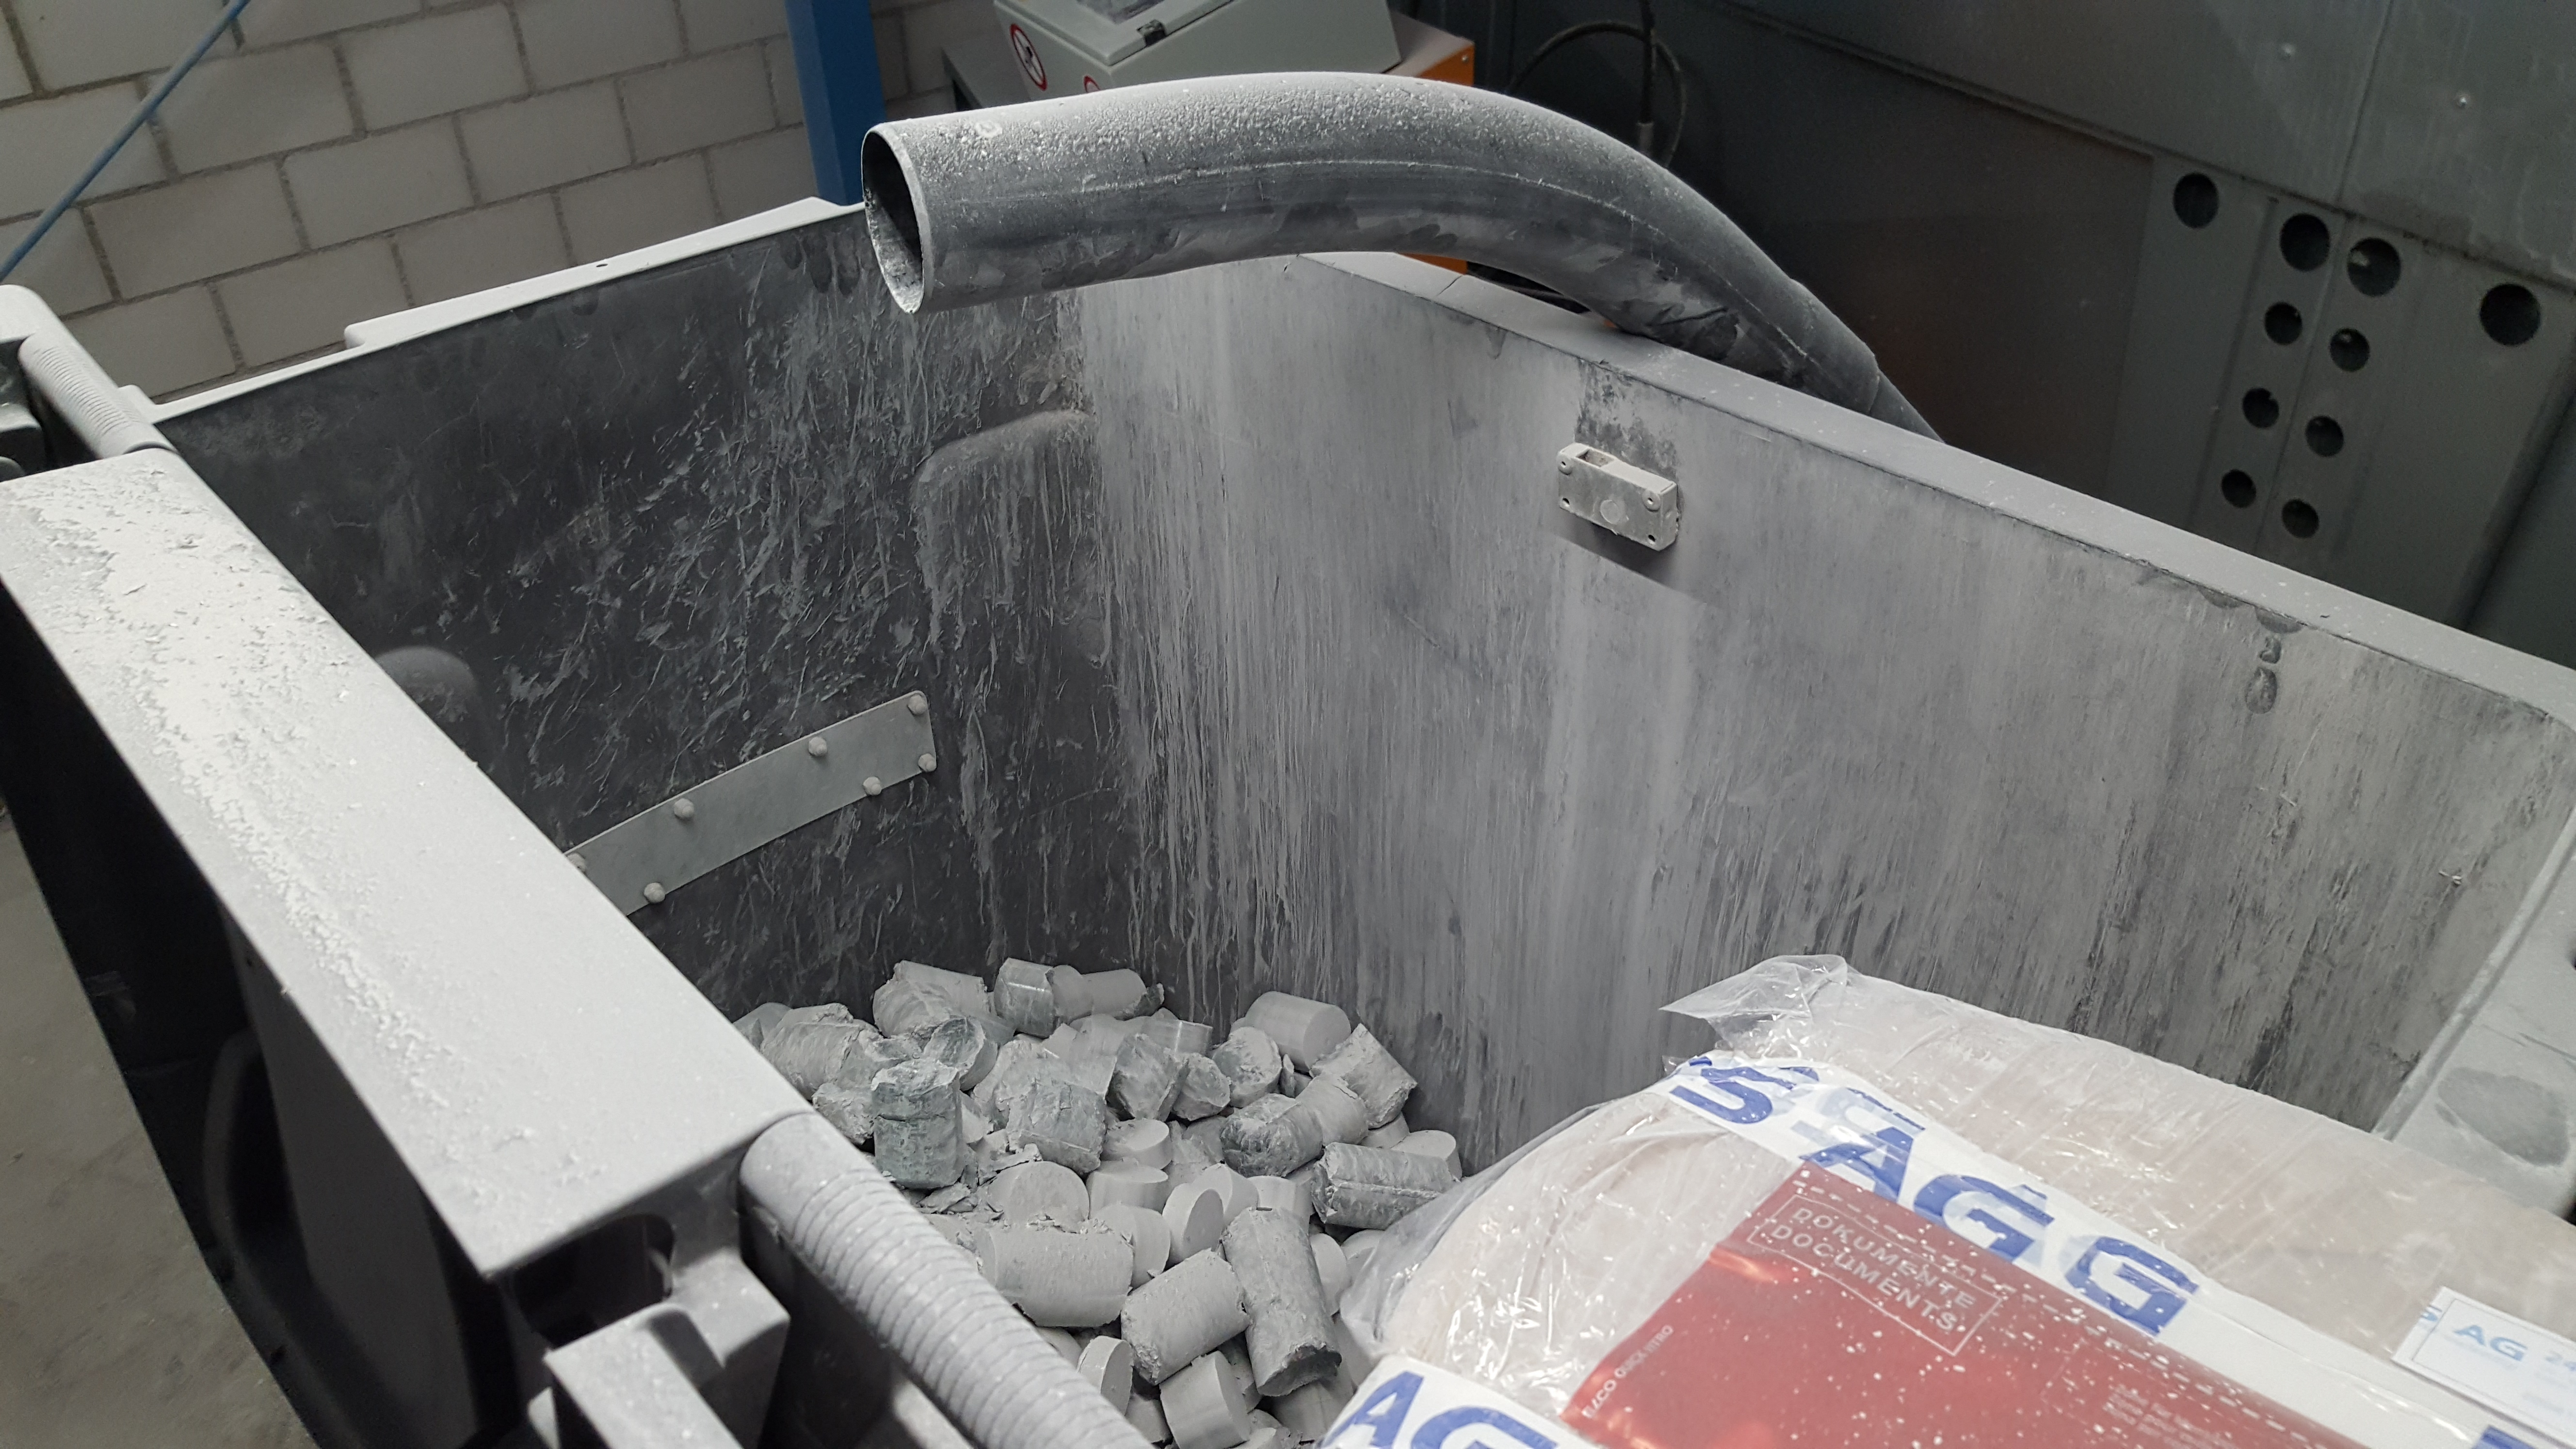
\includegraphics[width=0.4\textwidth]{images/papier_entsorgung_2.jpg}\label{fig:f2}}
  \caption{Paper disposal}
\end{figure}

Building off of the bar plot visualizations above and the characteristics of time series in \hyperlink{subsection3.3}{Section 3.3}, it is likely that the machines have a cyclical pattern. \hyperlink{figure.8}{Figure 8} is an hourly load profile heat map of the paper disposal machine. It is evident there is a daily periodicity from Monday-Friday with little to no demand on the weekend. The heat map indicates a daily and potential weekly pattern; though more data is needed to confirm the weekly periodicity hypothesis. 

\begin{figure}[h]
\centering
\graphicspath{ {./images/} }
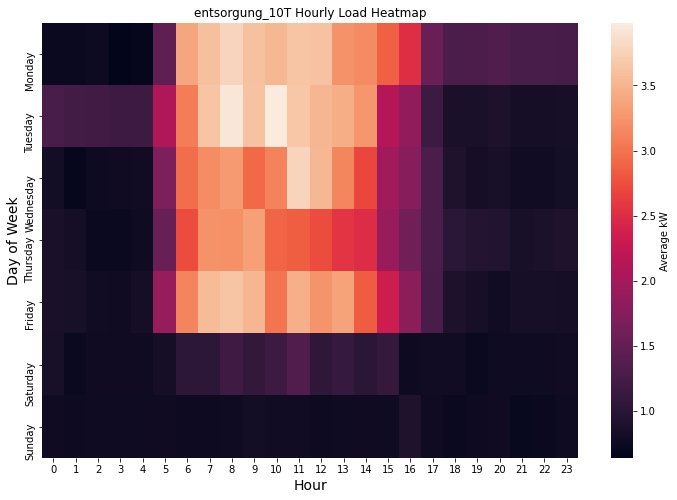
\includegraphics[scale=0.55]{images/entsorgung_hourly_heatmap.png}
\caption{Paper disposal hourly load profile. The color bar on the right indicates the average kW consumed for that hour over the $10$ day period.}
\end{figure}

Next, in \hyperlink{figure.9}{Figure 9}, a plot of the time series at a $10$ minute interval is visualized where 2021-10-08 is a Friday and 2021-10-18 is a Monday. The load profile shows a daily, and potentially sub-daily periodic pattern. Also, the $10$ days of data does not split into an even two weeks of data. Rather, there is only observations for one full production week. This inconsistency does not allow for an analysis or modeling of the weekly periodicity. 

\begin{figure}[h]
\centering
\graphicspath{ {./images/} }
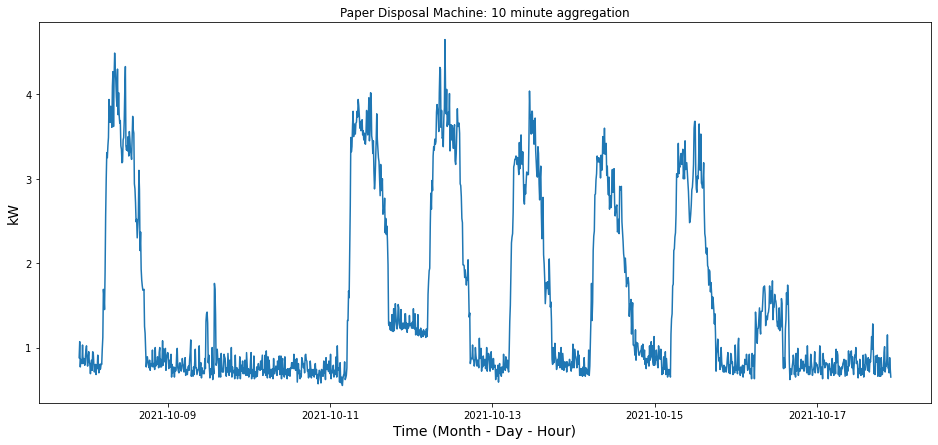
\includegraphics[scale=0.49]{images/entsorgung_10T_series.png}
\caption{Entire time series for the paper disposal machine.}
\end{figure}

Therefore, during the modeling phase, only the production week (2021-10-11 through 2021-10-15) is used. Using this time series, the periodicity is verified empirically using the ACF; as explained in \hyperlink{subsection.3.5.3}{Section 3.5.3}. Below, in \hyperlink{figure.10}{Figure 10}, the production week time series is visualized along with the respective ACF correlogram. 

\begin{figure}
    \centering
    \graphicspath{ {./images/} }
    \subfloat[a][a]{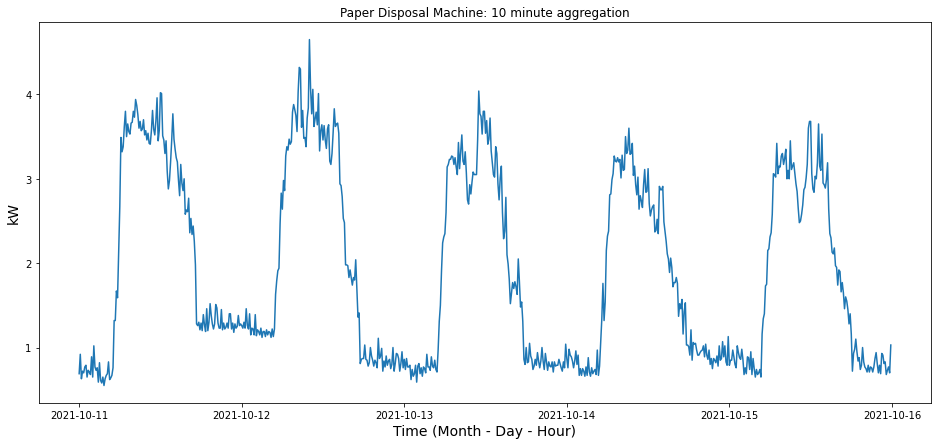
\includegraphics[width=1\textwidth]{images/entsorgung_10T_production_week.png}\label{fig:a}} \\
    \subfloat[b][b]{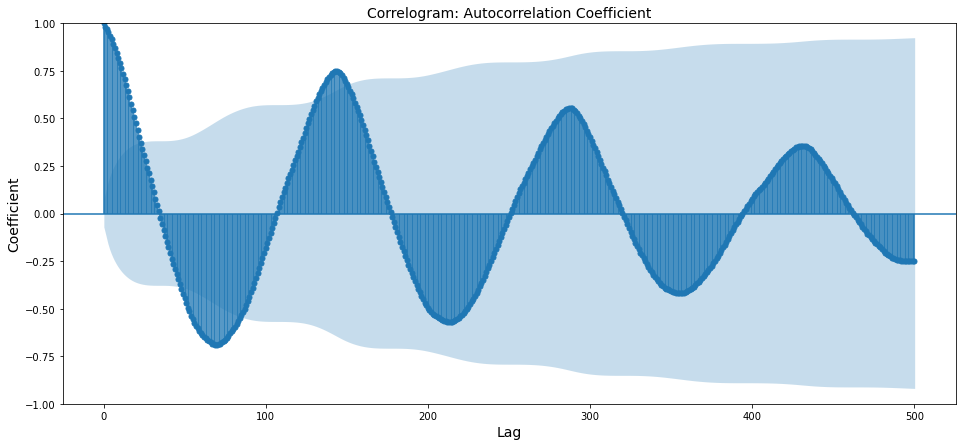
\includegraphics[width=1\textwidth]{images/entsorgung_10T_acf.png}\label{fig:b}}
    \caption{(a) Production week time series at $10$ minute aggregations. (b) ACF correlogram indicates significant periodic cycles at about $12$ and $24$ hours, respectively.} \label{fig:AB}
    \label{fig:my_label}
\end{figure}

Finally, the original time series is split into shorter time samples to gain a better visual understanding of the $12$Hz frequency.


\subsection{HIPE Industrial Energy}
Complementing CLEMAP's client machine-level data, a second source of data, the HIPE energy status data set \cite{HIPE}, will also be analyzed to ensure the scalability of the proposed methodologies in section 4. By developing the algorithms on a range of industrial equipment, the work can give vital feedback on the difficulties and opportunities to scale the deployment of models built on specific data sets to new data of similar applications. 

\subsection{HIPE Energy Open Dataset}

\begin{table}[htbp]
    \renewcommand{\arraystretch}{1.2}
    \centering
    \begin{tabular}{lcccccc}
    \hline
         Machine/Component & System & Amperes & Location & Floor & Purpose  \\
    \hline
    Gesamtmessung & & 1600 & Bau II & 0 & Main terminal \\
    Hauptluftung & HVAC & 250 & Bau II & -1 & Main ventilation \\
    Kältemaschiene & & 200 & Bau II & 1 & Refrigeration \\
    Drückmaschine & XL106 & 315 & Bau II & 2 & Printer \\
    UV Scan & XL106 & 160 & Bau II & 1 & undefined \\
    UV Sigmaline EG & & 315 & Bau II & 0 & undefined \\
    Stahl Folder & & 63 & Bau II & 0 & Steel folding \\
    Puderabsauger & R707LV & 25 & Bau II & 2 & Powder extraction \\
    Vari Air & R707LV & 100 & Bau II & 2 & undefined \\
    Trockner & R707LV & 160 & Bau II & 2 & Dryer \\
    UV Feinabgäng & & 125 & Bau II & 0 & UV fine particle extractor \\
    Papier Entsorgung & & 125 & Bau II & -1 & Paper disposal \\
    UV 1.0G & & 125 & Bau II & 1 & UV server room \\
    UV 2.0G & & 125 & Bau II & 2 & $2^{nd}$ floor \\
    UV 3.0G & & 125 & Bau II & 3 & $3^{rd}$ floor \\
    UV 4.0G & & 160 & Bau II & 4 & $4^{th}$ floor \\
    UV EG & & 125 & Bau II & 0 & UV ground floor \\
    \hline
    \end{tabular}
    \caption{List of items being metered by CLEMAP. A system may be composed of several machines, all of which are being metered.}
    \label{tab:my_label}
\end{table}

\subsection{Similarity and Differences of Data Sources}